\documentclass{standalone}

\usepackage{tikz}
    \usetikzlibrary{arrows.meta}
    \usetikzlibrary{calc}
    
\begin{document}
\begin{tikzpicture}
%\draw[help lines] (6,0) grid (17,5);
%\node[shift={(2.5,2.16)}] {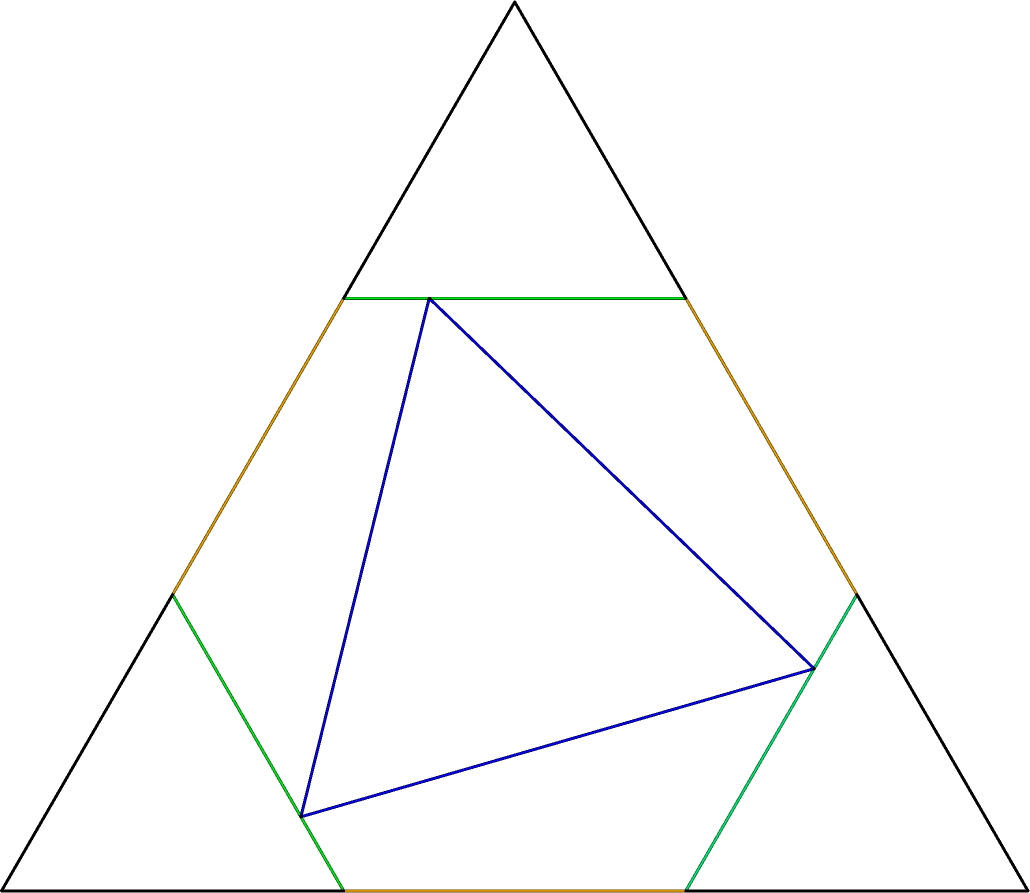
\includegraphics[width=5cm]{tr9p.png}};
\node[shift={(8.5,2.16)}] {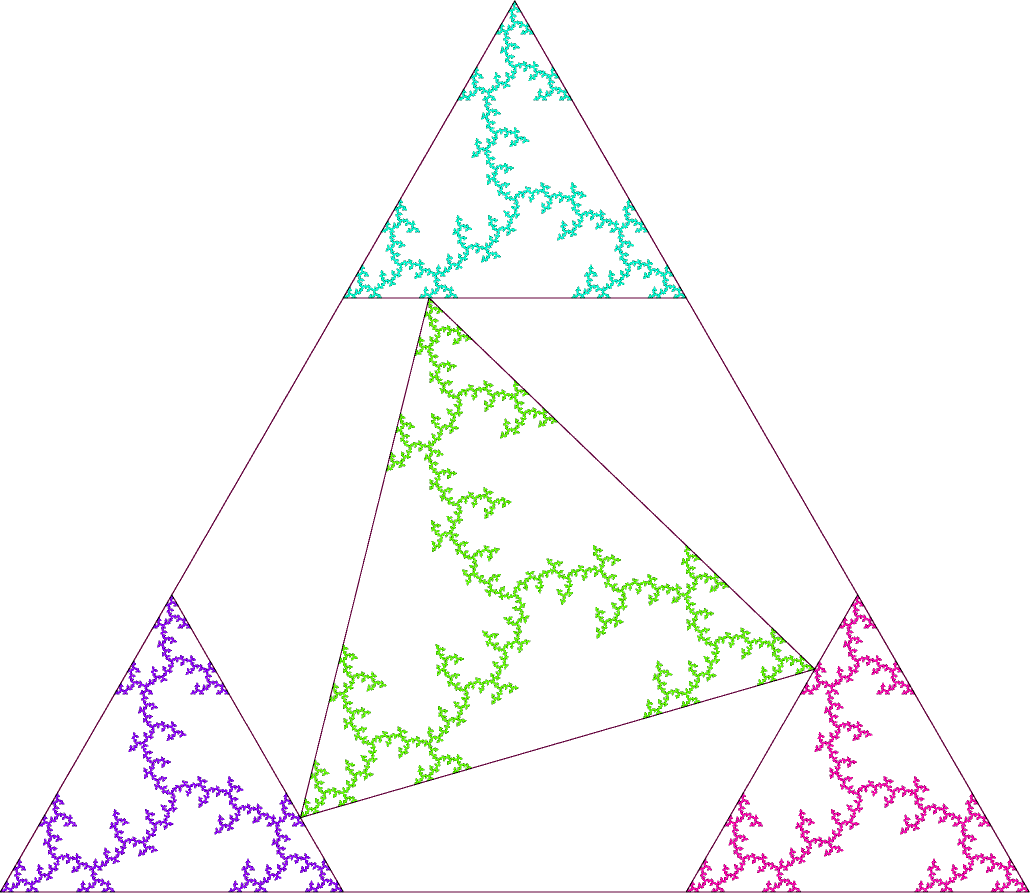
\includegraphics[width=5cm]{tr9k.png}};
\node[shift={(14.5,2.16)}] {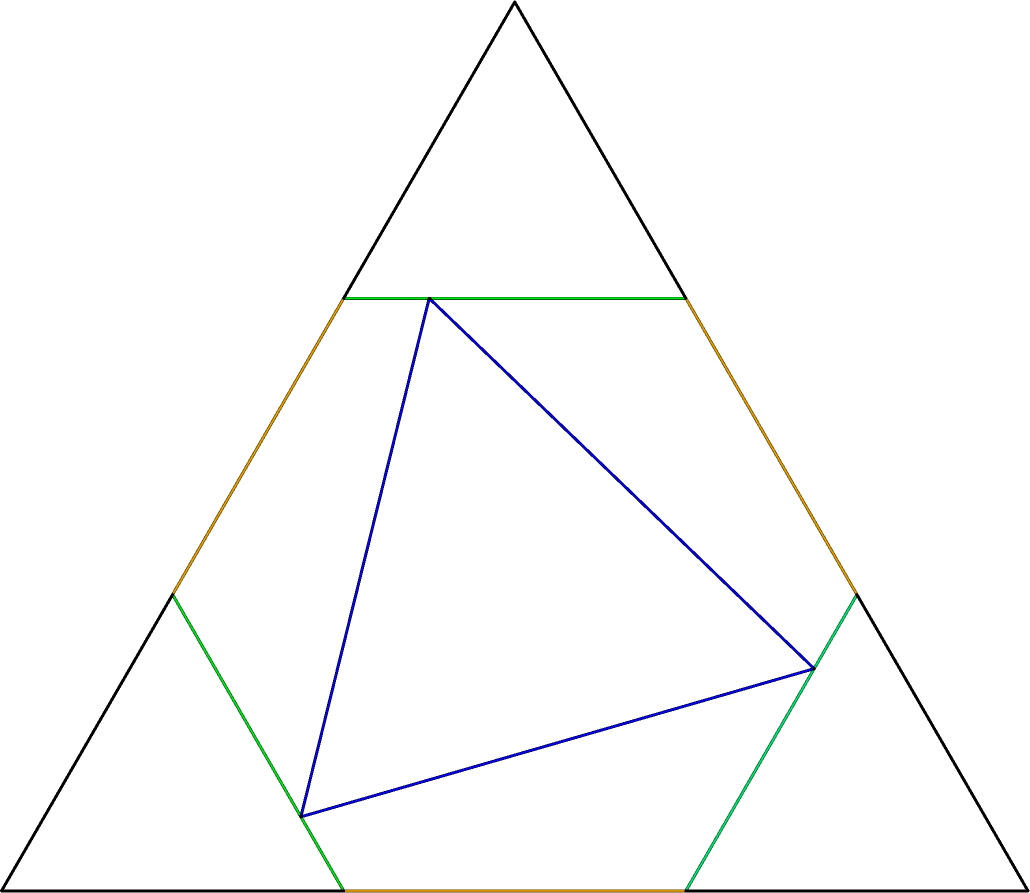
\includegraphics[width=5cm]{tr9p.png}};
\fill[red]
	(6,0)circle(0.7mm) ++(6,0)circle(0.7mm)
	(7.25,0)circle(0.7mm) ++(6,0)circle(0.7mm)
	(9.75,0)circle(0.7mm) ++(6,0)circle(0.7mm)
	(11,0)circle(0.7mm) ++(6,0)circle(0.7mm)
	(8.5,4.33)circle(0.7mm) ++(6,0)circle(0.7mm)
	(6.625,1.08)circle(0.7mm) ++(6,0)circle(0.7mm)
	(10.375,1.08)circle(0.7mm) ++(6,0)circle(0.7mm)
	(7.875,3.25)circle(0.7mm) ++(6,0)circle(0.7mm)
	(9.125,3.25)circle(0.7mm) ++(6,0)circle(0.7mm);

\fill[blue]
	(7.45,0.36)circle(0.7mm) ++(6,0)circle(0.7mm)
	(9.95,1.08)circle(0.7mm) ++(6,0)circle(0.7mm)
	(8.08,2.87)circle(0.7mm) ++(6,0)circle(0.7mm);
\footnotesize
\node[] at (12.8,0.4) {$S_1(K)$};
\node[] at (16.2,0.4) {$S_2(K)$};
\node[] at (14.5,3.3) {$S_3(K)$};
\node[] at (14.5,1.4) {$S_4(K)$};
\footnotesize
\node[below] at (12,0) {$\overline{1}$};
\node[below] at (13.25,0)  {$\overline{12}$};
\node[below] at (15.75,0) {$\overline{21}$};
\node[below] at (17,0)  {$\overline{2}$};
\node[above] at (14.5,4.33)  {$\overline{3}$};
\node[left] at (12.625,1.08)  {$\overline{13}$};
\node[right] at (16.375,1.08)  {$\overline{23}$};
\node[left] at (13.875,3.25)  {$\overline{31}$};
\node[right] at (15.125,3.25)  {$\overline{32}$};

\node[right] at (13.45,0.26) {$4\overline{1};1\overline{23}$};
\node[left] at (15.95,1.18) {$4\overline{2};2\overline{31}$};
\node[below right] at (14.18,2.97) {$4\overline{3};3\overline{12}$};

\end{tikzpicture}
\end{document}